\chapter{Mengukur Panjang}\label{ch:g2:measuring-length}

Dua pintu, di dua rumah yang berbeda: mana yang lebih tinggi? Kamu
tidak dapat menggotong sebuah pintu melintasi kota untuk
menyandingkannya dengan pintu yang lain. Tahun lalu kita membandingkan
benda secara berdampingan; tahun ini kita belajar tipu muslihat
terbesar ilmu pengetahuan --- mengubah panjang menjadi sebuah
\emph{bilangan} yang dapat bepergian.

\section{Membandingkan tanpa bilangan}

\begin{example}[Berdampingan]\label{ex:g2:measuring-length:sidebyside}
Untuk mencari pensil yang lebih panjang di antara dua pensil,
tegakkan keduanya bersama di atas meja: yang menonjol keluar itulah
pemenangnya. Untuk membandingkan tinggimu dengan tinggi seorang
teman, berdirilah saling membelakangi. Cara ini bekerja dengan indah
--- selama kedua benda dapat dipertemukan.
\end{example}

\begin{example}[Tipu muslihat tali]\label{ex:g2:measuring-length:string}
Kedua pintu tidak dapat bertemu --- tetapi seutas tali dapat
mengunjungi keduanya. Bentangkan seutas tali pada pintu pertama dan
potonglah tepat setinggi pintu itu. Bawalah tali itu ke pintu kedua:
kalau talinya terlalu pendek, pintu kedua lebih tinggi. Tali itu
membawa tinggi pintu pertama menyeberangi kota. Satu langkah lebih
baik lagi: bagaimana kalau tingginya dapat kita kirim lewat
\emph{surat}? Untuk itu kita memerlukan bilangan.
\end{example}

\section{Mengukur dengan langkah dan jengkal}

\begin{definition}[Mengukur panjang]\label{def:g2:measuring-length:measure}
Untuk \emph{mengukur}\index{mengukur} sebuah panjang, kita menghitung
berapa kali sebuah \emph{satuan}\index{satuan} pilihan --- satu
langkah, satu jengkal, sebatang tongkat kecil --- termuat di
sepanjang benda itu, ujung bertemu ujung, tanpa celah dan tanpa
tumpang tindih. Jawabannya berupa bilangan bersatuan: ``ruangan ini
panjangnya $12$ langkah.''
\end{definition}

\begin{example}[Cobalah: langkahi ruanganmu]\label{ex:g2:measuring-length:pace}
Seberangi kamar tidurmu dengan tumit bertemu ujung jari kaki, sambil
menghitung panjang telapak kakimu. Mintalah orang dewasa melakukan hal
yang sama. Kamu mungkin menghitung $18$ telapak dan orang dewasa itu
hanya $12$ --- untuk \emph{ruangan yang sama}! Tidak ada yang salah
hitung: telapak kakimu lebih pendek, sehingga lebih banyak yang
termuat. Pengukuran dengan telapak kaki\emph{ku} tidak dapat diperiksa
dengan telapak kaki\emph{mu}.
\end{example}

\begin{omfigure}
\begin{tikzpicture}[scale=0.8]
  \draw[thick] (0,1.6) -- (9,1.6);
  \foreach \i in {0,...,11} {
    \draw[omDef, thick] (\i*0.75,1.6) rectangle ++(0.75,0.28);
  }
  \node[right, font=\small] at (9.2,1.74) {si anak: $12$ telapak kecil};
  \draw[thick] (0,0) -- (9,0);
  \foreach \i in {0,...,7} {
    \draw[omThm, thick] (\i*1.125,0) rectangle ++(1.125,0.28);
  }
  \node[right, font=\small] at (9.2,0.14) {orang dewasa: $8$ telapak besar};
\end{tikzpicture}

{\small Dinding yang sama, dilangkahi dua kali: $12$ telapak kecil,
atau $8$ telapak besar. Telapak berbeda, bilangan berbeda ---
dindingnya sendiri tidak berubah.}
\end{omfigure}

\begin{remark}[Pertengkaran di pasar]\label{rem:g2:measuring-length:argument}
Selama waktu yang lama, orang memang \omterm{def:g2:measuring-length:measure}{mengukur} dengan telapak kaki, ibu
jari, dan depa, dan pasar pun ramai oleh pertengkaran: telapak kaki
siapa? milik pedagang yang jangkung atau milik pembeli yang pendek?
Jalan keluarnya, yang disepakati di seluruh dunia, adalah memilih
\emph{satu} \omterm{def:g2:measuring-length:measure}{satuan} untuk semua orang --- \omterm{def:g2:measuring-length:measure}{satuan} yang bukan milik tubuh
siapa pun.
\end{remark}

\section{Sentimeter dan meter}

\begin{definition}[Sentimeter dan meter]\label{def:g2:measuring-length:units}
\omterm{def:g2:measuring-length:measure}{Satuan} panjang yang kecil, kira-kira selebar kuku jari, disebut
\emph{sentimeter}\index{sentimeter} (ditulis \unit{cm}); \omterm{def:g2:measuring-length:measure}{satuan} ini
tercetak pada setiap penggaris. \omterm{def:g2:measuring-length:measure}{Satuan} yang besar, tepat $100$
sentimeter, sepanjang satu langkah yang sangat lebar, disebut
\emph{meter}\index{meter} (ditulis \unit{m}). \omterm{def:g2:measuring-length:measure}{Satuan} ini sama bagi
semua orang di Bumi: \qty{20}{cm} milikmu dan \qty{20}{cm} milikku
tepat sama besar.
\end{definition}

\begin{omfigure}
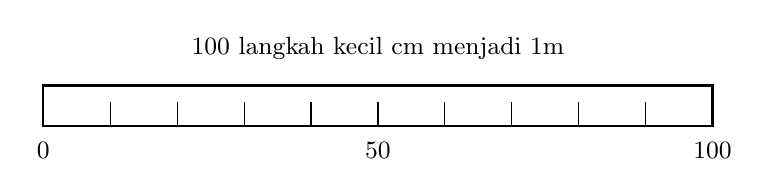
\begin{tikzpicture}[scale=0.85]
  \draw[thick] (0,0.5) rectangle (10,1.1);
  \foreach \i in {1,...,9} {
    \draw (\i,0.5) -- (\i,0.85);
  }
  \node[below, font=\small] at (0,0.4) {$0$};
  \node[below, font=\small] at (5,0.4) {$50$};
  \node[below, font=\small] at (10,0.4) {$100$};
  \node[above, font=\small] at (5,1.35)
    {$100$ langkah kecil \unit{cm} menjadi \qty{1}{m}};
\end{tikzpicture}

{\small Tongkat semeter: seratus \omterm{def:g2:measuring-length:units}{sentimeter} berderet. Tanda-tandanya
memungkinkan kita menghitungnya dengan cepat, bukan satu per satu.}
\end{omfigure}

\begin{method}[Mengukur dengan penggaris]\label{met:g2:measuring-length:ruler}
\begin{enumerate}
  \item Letakkan penggaris di sepanjang benda, menempel padanya;
  \item tempatkan \emph{tanda nol} penggaris tepat di salah satu ujung
        benda --- bukan tepi penggarisnya, melainkan angka $0$;
  \item bacalah bilangan di ujung yang lain: itulah panjangnya dalam
        \omterm{def:g2:measuring-length:units}{sentimeter}.
\end{enumerate}
Kalau ujungnya jatuh di antara dua tanda, katakan ``antara \qty{7}{cm}
dan \qty{8}{cm}, lebih dekat ke $8$'' --- kata yang jujur lebih baik
daripada bilangan yang dikarang.
\end{method}

\begin{omfigure}
\begin{tikzpicture}[scale=0.85]
  \draw[thick] (0,0) rectangle (8.4,0.7);
  \foreach \i in {0,...,12} {
    \draw (0.2+\i*0.65,0) -- (0.2+\i*0.65,0.3);
    \node[below, font=\footnotesize] at (0.2+\i*0.65,0) {\i};
  }
  \draw[thick, fill=omMeth, fill opacity=0.5]
    (0.2,1.0) rectangle (5.4,1.45);
  \node[font=\small] at (2.8,1.22) {krayon};
  \draw[dashed, omExo] (0.2,0.35) -- (0.2,1.0);
  \draw[dashed, omExo] (5.4,0.35) -- (5.4,1.0);
  \node[above, font=\small] at (5.4,1.5) {terbaca $8$: \qty{8}{cm}};
\end{tikzpicture}

{\small Membaca penggaris: tanda nol di salah satu ujung krayon, lalu
baca ujung yang lain. Krayon ini panjangnya \qty{8}{cm}.}
\end{omfigure}

\begin{omfigure}
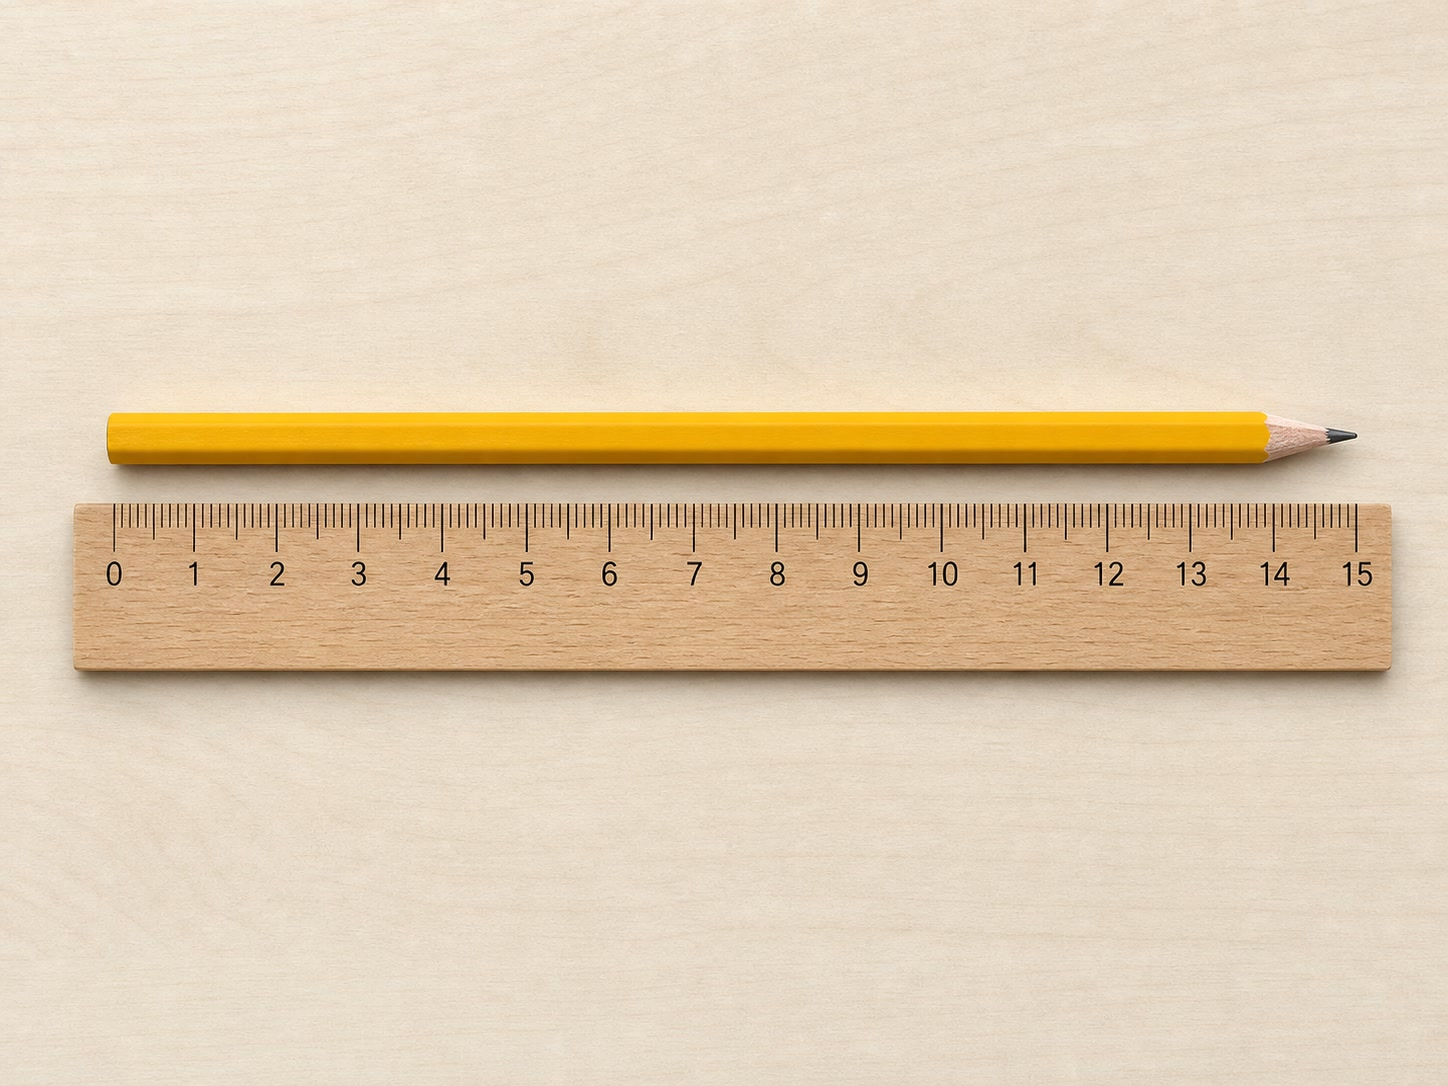
\includegraphics[width=0.52\linewidth]{images/book1/ai/g2-measuring-ruler.jpg}

{\small Pengukuran yang dilakukan dengan benar: ujung pensil duduk tepat pada tanda nol penggaris.}
\end{omfigure}

\begin{example}[Satuan mana untuk pekerjaan mana?]\label{ex:g2:measuring-length:whichunit}
Benda kecil seperti kumbang, perangko, atau tanganmu diukur dalam
\omterm{def:g2:measuring-length:units}{sentimeter}. Benda besar seperti koridor, bus, atau kolam renang diukur
dalam \omterm{def:g2:measuring-length:units}{meter}: kolam itu panjangnya \qty{25}{m} --- bayangkan
menghitungnya dalam lebar kuku! Memilih \omterm{def:g2:measuring-length:measure}{satuan} yang masuk akal adalah
separuh dari pekerjaan \omterm{def:g2:measuring-length:measure}{mengukur}.
\end{example}

\begin{example}[Taksir dulu, baru periksa]\label{ex:g2:measuring-length:estimate}
Sebelum \omterm{def:g2:measuring-length:measure}{mengukur}, para pemain menebak: berapa panjang meja dapur?
Ayah berkata \qty{2}{m}, Lina berkata \qty{1}{m} lebih sedikit. Lalu
tongkat semeter yang memutuskan: \qty{1}{m} dan hampir setengahnya
lagi --- satu angka untuk Lina. Menebak lebih dahulu melatih matamu;
\omterm{def:g2:measuring-length:measure}{mengukur} membuat semua orang jujur.
\end{example}

\section{Latihan}

\begin{exercise}[$\star$]\label{exo:g2:measuring-length:1}
Bagaimana kamu dapat membandingkan tinggimu dengan tinggi seorang
teman tanpa penggaris? Dan dengan tinggi teman yang tinggal di kota
lain?
\end{exercise}

\begin{exercise}[$\star$]\label{exo:g2:measuring-length:2}
Mara \omterm{def:g2:measuring-length:measure}{mengukur} ruang kelas dengan langkah dan mendapat $20$; gurunya
mendapat $14$. Siapa yang salah hitung? Jelaskan.
\end{exercise}

\begin{exercise}[$\star$]\label{exo:g2:measuring-length:3}
Apa istimewanya \omterm{def:g2:measuring-length:units}{sentimeter} dibandingkan dengan panjang telapak kaki
atau jengkal? Mengapa orang menyepakatinya?
\end{exercise}

\begin{exercise}[$\star$]\label{exo:g2:measuring-length:4}
\omterm{def:g2:measuring-length:measure}{Satuan} mana yang lebih cocok, \unit{cm} atau \unit{m}: panjang seekor
semut; \ tinggi sebuah pintu; \ panjang halaman sekolah; \ lebar buku
ini?
\end{exercise}

\begin{exercise}[$\star$]\label{exo:g2:measuring-length:5}
Tim menempelkan tepi penggarisnya --- bukan tanda nol --- pada ujung
pensilnya, lalu membaca \qty{13}{cm}. Benarkah pensilnya sepanjang
\qty{13}{cm}? Apa yang ia lupakan dari
\cref{met:g2:measuring-length:ruler}?
\end{exercise}

\begin{exercise}[$\star$]\label{exo:g2:measuring-length:6}
Ukurlah dengan penggaris: lebar tanganmu; \ panjang sebuah sendok;
\ tinggi sebuah cangkir. Tulislah setiap jawaban dengan \omterm{def:g2:measuring-length:measure}{satuannya}.
\end{exercise}

\begin{exercise}[$\star$]\label{exo:g2:measuring-length:7}
Sebuah pintu tingginya \qty{2}{m}. Berapa sentimeterkah itu? (Ingat:
\qty{1}{m} adalah $100$ \unit{cm}.)
\end{exercise}

\begin{exercise}[$\star$]\label{exo:g2:measuring-length:8}
Tebak dulu, lalu ukurlah: berapa \omterm{def:g2:measuring-length:units}{meter} panjang tempat tidurmu? Apakah
tebakanmu terlalu besar, terlalu kecil, atau hampir tepat?
\end{exercise}

\begin{exercise}[$\star\star$]\label{exo:g2:measuring-length:9}
Sehelai pita panjangnya \qty{45}{cm}, pita lain \qty{38}{cm}. Mana
yang lebih panjang, dan berapa \omterm{def:g2:measuring-length:units}{sentimeter} selisihnya? Dapatkah kamu
memutuskannya \emph{tanpa} bilangan? Cara mana yang lebih mudah
ditulis dalam sebuah surat?
\end{exercise}

\begin{exercise}[$\star\star$]\label{exo:g2:measuring-length:10}
Kakek berkata: ``Kebunku panjangnya $30$ langkah.'' Jelaskan kepada
Kakek, dengan baik-baik, mengapa ``$30$ langkah'' tidak dapat
diperiksa orang lain, dan apa yang sebaiknya ia pakai. Apa yang akan
terjadi kalau anak kecil melangkahi kebun yang sama?
\end{exercise}
